\section{Hard Disk Drive (HDD) Technology}

A Hard Disk Drive (HDD) is an electro-mechanical, non-volatile computer data storage device that utilizes magnetic storage to store and retrieve digital data \cite{wiki_hdd}. Unlike volatile RAM, HDDs retain data even when the power is turned off, making them the primary choice for long-term storage of operating systems, applications, and user files \cite{gfg_hdd_memory, gfg_storage_structure}.

\subsection{Physical Infrastructure}


\begin{enumerate}[label=\roman*.]
    \item \textbf{Platters and Spindle:} The physical structure of an HDD consists of rigid, rapidly rotating circular disks called platters, which are coated with magnetic material \cite{wiki_hdd, gfg_hdd_memory}.

    \item \textbf{Read/Write Heads:} Data is accessed via read/write heads positioned on a moving actuator arm that traverses the platter surfaces in a random-access manner, allowing individual blocks of data to be retrieved in any order \cite{wiki_hdd, gfg_hdd_memory}.
    
    \item \textbf{Mechanical Speed:} These platters are mounted on a central spindle that rotates at high speeds, typically ranging from 4,200 to 15,000 RPM \cite{gfg_hdd_memory, wiki_hdd}.
    
\end{enumerate}


\vspace{1 in}
\begin{figure}[H]
    \centering
    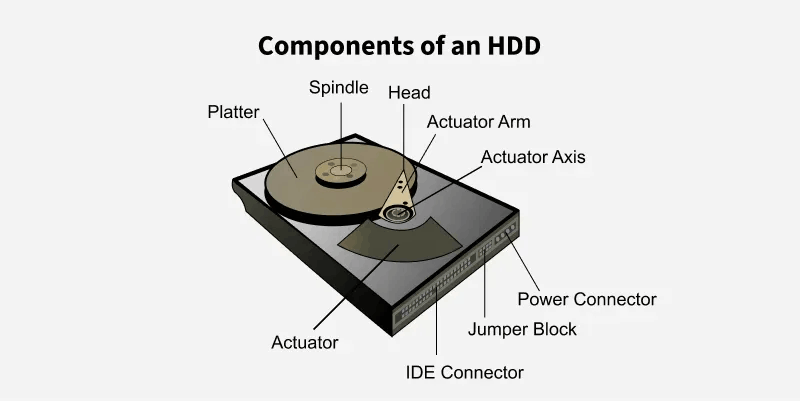
\includegraphics[width=1\linewidth]{HDD Components.png}
    \caption{Internal Components of HDD \cite{gfg_hdd_memory}}
    \label{fig:inside HDD}
\end{figure}